% Scenario figure (Fig. 1). Build: xelatex fig0_scene.tex (next to scene_icons.tex, bev_frame.png, bev_feat.png).
% The left panel is a real nuScenes-mini LiDAR sweep rendered top-down by render_bev.py; the texture on the
% map's front face (bev_feat.png, same script) illustrates one BEV feature channel on the 180 x 180 grid.
% Text in Carlito (metric-compatible with the Calibri of the plots). Icons: Lucide (ISC) and Tabler (MIT)
% outline icons converted to TikZ paths by svg2tikz.py; see ICONS-LICENSE.txt.
\documentclass[border=0pt]{standalone}
\usepackage{fontspec}
\setmainfont{Carlito}
\usepackage{tikz}
\usetikzlibrary{arrows.meta,fit,backgrounds}
% Generated by svg2tikz.py from Lucide (ISC) and Tabler (MIT) icons; see ICONS-LICENSE.txt.
\expandafter\def\csname ico@Lcamera\endcsname{\draw (13.997,4) .. controls (14.732,4) and (15.408,4.403) .. (15.757,5.05) -- (16.243,5.95) .. controls (16.592,6.597) and (17.268,7) .. (18.003,7) -- (20,7) .. controls (21.105,7) and (22,7.895) .. (22,9) -- (22,18) .. controls (22,19.105) and (21.105,20) .. (20,20) -- (4,20) .. controls (2.895,20) and (2,19.105) .. (2,18) -- (2,9) .. controls (2,7.895) and (2.895,7) .. (4,7) -- (5.997,7) .. controls (6.731,7) and (7.406,6.598) .. (7.756,5.952) -- (8.245,5.048) .. controls (8.595,4.402) and (9.27,4) .. (10.004,4) -- cycle; \draw (12,13) circle (3);}
\expandafter\def\csname ico@Lgpu\endcsname{\draw (2,17) -- (20,17) .. controls (21.105,17) and (22,16.105) .. (22,15) -- (22,7) .. controls (22,5.895) and (21.105,5) .. (20,5) -- (2,5); \draw (2,21) -- (2,3); \draw (7,17) -- (7,20) .. controls (7,20.552) and (7.448,21) .. (8,21) -- (13,21) .. controls (13.552,21) and (14,20.552) .. (14,20) -- (14,17); \draw (16,11) circle (2); \draw (8,11) circle (2);}
\expandafter\def\csname ico@Tobjectscan\endcsname{\draw (8,10) .. controls (8,8.895) and (8.895,8) .. (10,8) -- (14,8) .. controls (15.105,8) and (16,8.895) .. (16,10) -- (16,14) .. controls (16,15.105) and (15.105,16) .. (14,16) -- (10,16) .. controls (8.895,16) and (8,15.105) .. (8,14) -- (8,10); \draw (3,7) -- (3,5) .. controls (3,3.895) and (3.895,3) .. (5,3) -- (7,3); \draw (3,17) -- (3,19) .. controls (3,20.105) and (3.895,21) .. (5,21) -- (7,21); \draw (17,3) -- (19,3) .. controls (20.105,3) and (21,3.895) .. (21,5) -- (21,7); \draw (17,21) -- (19,21) .. controls (20.105,21) and (21,20.105) .. (21,19) -- (21,17);}
\expandafter\def\csname ico@Lcrosshair\endcsname{\draw (12,12) circle (10); \draw (22,12) -- (18,12); \draw (6,12) -- (2,12); \draw (12,6) -- (12,2); \draw (12,22) -- (12,18);}
\expandafter\def\csname ico@Lroute\endcsname{\draw (6,19) circle (3); \draw (9,19) -- (17.5,19) .. controls (19.433,19) and (21,17.433) .. (21,15.5) .. controls (21,13.567) and (19.433,12) .. (17.5,12) -- (6.5,12) .. controls (4.567,12) and (3,10.433) .. (3,8.5) .. controls (3,6.567) and (4.567,5) .. (6.5,5) -- (15,5); \draw (18,5) circle (3);}
\expandafter\def\csname ico@Ldatabase\endcsname{\draw (12,5) ellipse (9 and 3); \draw (3,5) -- (3,19) .. controls (3,20.657) and (7.029,22) .. (12,22) .. controls (16.971,22) and (21,20.657) .. (21,19) -- (21,5); \draw (3,12) .. controls (3,13.657) and (7.029,15) .. (12,15) .. controls (16.971,15) and (21,13.657) .. (21,12);}
\expandafter\def\csname ico@Lcirclehelp\endcsname{\draw (12,12) circle (10); \draw (9.09,9) .. controls (9.575,7.62) and (10.985,6.791) .. (12.427,7.039) .. controls (13.869,7.286) and (14.922,8.537) .. (14.92,10) .. controls (14.92,12) and (11.92,13) .. (11.92,13); \fill (12,17) circle (1);}


\definecolor{ink}{HTML}{1F2933}\definecolor{sub}{HTML}{5F6B7A}\definecolor{line}{HTML}{B4BDC7}
\definecolor{panel}{HTML}{F3F6FA}\definecolor{tile}{HTML}{E9EEF4}\definecolor{night}{HTML}{0D1520}
\definecolor{bimD}{HTML}{1F4E8C}\definecolor{bimA}{HTML}{3A73C0}
\definecolor{frD}{HTML}{B07A12}\definecolor{frA}{HTML}{E9B23A}\definecolor{frT}{HTML}{F8E3AE}\definecolor{frF}{HTML}{FFF6DF}
\definecolor{coral}{HTML}{C8414B}\definecolor{iconT}{HTML}{E6EEF8}

\newcommand{\fs}[1]{\fontsize{#1}{#1}\selectfont}
\newcommand{\var}[1]{\textit{#1}}
\newdimen\icou
\newcommand{\icon}[4][]{%
  \icou=\dimexpr #4pt/24\relax
  \begin{scope}[shift={#3},x=\icou,y=-\icou,shift={(-12,-12)},line width=1.8\icou,
                line cap=round,line join=round,#1]
    \csname ico@#2\endcsname
  \end{scope}}
\tikzset{flow/.style={-{Latex[length=3pt,width=2.6pt]},line width=.65pt,line cap=round}}

\begin{document}
\begin{tikzpicture}[x=1pt,y=1pt,font=\fs{6.6},text=ink]
\useasboundingbox (0,0) rectangle (252,92);
\def\yc{52}% the flow line: sensors -> map -> readers

% ---- frame k as the LiDAR sees it: one nuScenes sweep, 72 m across, ego vehicle at the center ----
\fill[black,opacity=.10,rounded corners=3.5pt] (1.7,2.6) rectangle (85.7,86.6);
\begin{scope}
  \clip[rounded corners=3pt] (1,3.4) rectangle (85,87.4);
  \node[anchor=south west,inner sep=0pt] at (1,3.4) {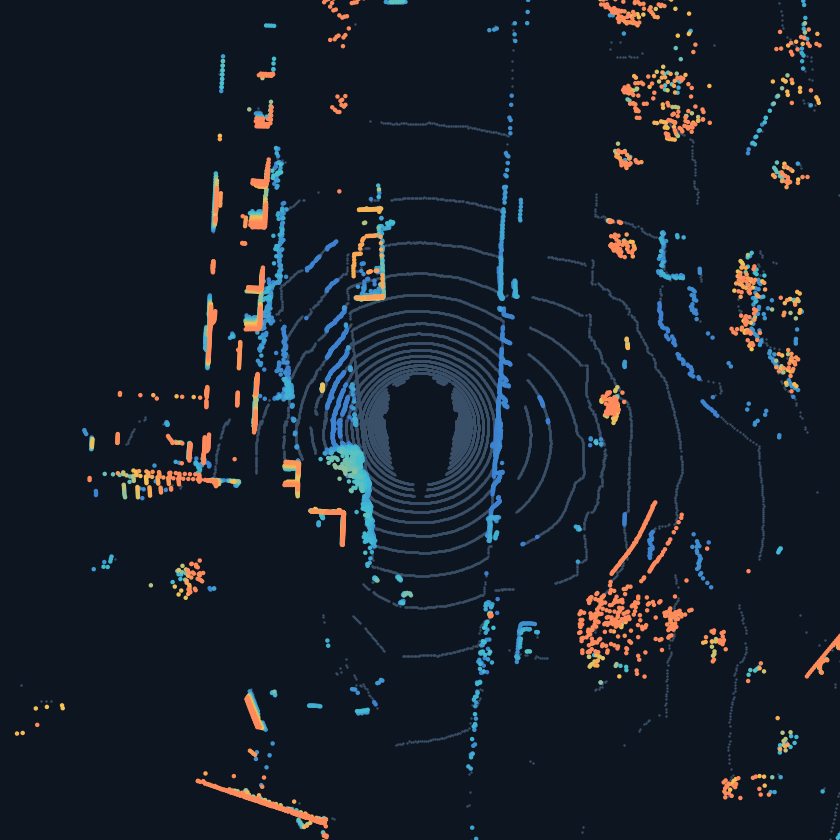
\includegraphics[width=84pt,height=84pt]{bev_frame.png}};
  \foreach \i in {1,...,11}{\draw[white,opacity=.07,line width=.3pt] (1+7*\i,3.4) -- (1+7*\i,87.4) (1,3.4+7*\i) -- (85,3.4+7*\i);}
\end{scope}
\fill[bimA,draw=white,line width=.35pt,rounded corners=.8pt] (41.5,42.3) rectangle (44.5,48.5);
\fill[white,opacity=.9] (41.95,46.0) rectangle (44.05,47.1);
\node[anchor=north west,fill=night,fill opacity=.7,text opacity=1,text=white,font=\fs{6.1},
      inner xsep=2.2pt,inner ysep=1.6pt,rounded corners=1.5pt] at (3.5,84.9) {LiDAR, frame \var{k}};
\fill[night,opacity=.7,rounded corners=1.5pt] (3.5,5.9) rectangle (29.6,12.5);
\draw[white,line width=.6pt] (5.8,9.2) -- (17.47,9.2);
\draw[white,line width=.45pt] (5.8,8.1) -- (5.8,10.3) (17.47,8.1) -- (17.47,10.3);
\node[anchor=west,text=white,font=\fs{5.6},inner sep=0pt] at (19.3,9.3) {10\,m};

% ---- fusion (with the six cameras) ----
\draw[flow,sub,line width=.75pt] (87.6,\yc) -- (100.4,\yc);
\filldraw[line,fill=white,line width=.5pt] (94,\yc+8.2) circle (4.7);
\icon[draw=sub]{Lcamera}{(94,\yc+8.2)}{6.4}
\node[font=\fs{5.9}\itshape,text=sub] at (94,\yc-5.4) {fusion};

% ---- the shared BEV map: one tensor, 512 channels on a 180 x 180 grid, in GPU memory ----
\fill[black,opacity=.06,rounded corners=3.5pt] (102.7,15.9) rectangle (171.7,86.7);
\shade[top color=white,bottom color=panel,rounded corners=3pt] (102,16.6) rectangle (171,87.4);
\draw[line,line width=.55pt,rounded corners=3pt] (102,16.6) rectangle (171,87.4);
\icon[draw=sub]{Lgpu}{(108.4,81.4)}{7.2}
\node[anchor=west,inner sep=0pt,font=\fs{5.9},text=sub] at (113.2,81.4) {GPU memory};
% channel slices, back to front; the front one carries a feature texture
\def\s{24}\def\ox{111.5}\def\oy{40}\def\dx{2.6}\def\dy{2.1}
\foreach \k/\c in {4/frA!45,3/frA!32,2/frT,1/frT!70!white}{
  \filldraw[fill=\c,draw=frD,line width=.42pt] ({\ox+\k*\dx},{\oy+\k*\dy}) rectangle ++(\s,\s);}
\begin{scope}
  \clip (\ox,\oy) rectangle ++(\s,\s);
  \node[anchor=south west,inner sep=0pt] at (\ox,\oy) {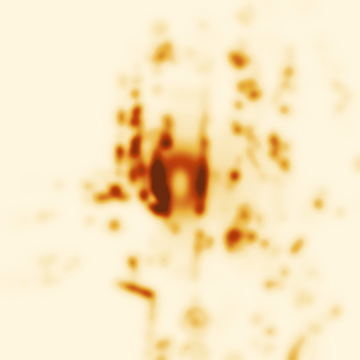
\includegraphics[width=24pt,height=24pt]{bev_feat.png}};
\end{scope}
\draw[frD,line width=.55pt] (\ox,\oy) rectangle ++(\s,\s);
\node[font=\fs{5.4},text=sub] at (\ox+\s/2,\oy-3.4) {180};
\node[font=\fs{5.4},text=sub,rotate=90] at (\ox-3.4,\oy+\s/2) {180};
\node[font=\fs{5.4},text=sub,rotate=39] at (\ox+4.6,\oy+\s+7.6) {512};
\node[font=\fs{6.6}\bfseries] at (136.5,30.2) {BEV map, frame \var{k}};
\node[inner sep=1.1pt,inner xsep=2.2pt,font=\fs{5.5}\bfseries,text=frD,fill=frT,rounded corners=2pt] at (136.5,22.4) {63.3\,MiB};

% ---- four reader processes, each on its own schedule ----
\foreach \y in {80.05,61.35,42.65,23.95}{
  \draw[flow,frD,rounded corners=2.6pt] (146.8,\yc) -- (177,\yc) -- (177,\y) -- (183.4,\y);}
\filldraw[frD,draw=white,line width=.4pt] (146.8,\yc) circle (1.5pt);
\foreach \y/\ic/\t in {80.05/Tobjectscan/3D detection,61.35/Lcrosshair/tracking,42.65/Lroute/motion planning,23.95/Ldatabase/recording}{
  \fill[black,opacity=.07,rounded corners=2.8pt] (185.1,\y-7.95) rectangle (251.6,\y+6.75);
  \draw[line,line width=.5pt,fill=white,rounded corners=2.5pt] (184.5,\y-7.35) rectangle (251,\y+7.35);
  \fill[iconT,rounded corners=2pt] (187,\y-5) rectangle (197,\y+5);
  \icon[draw=bimD]{\ic}{(192,\y)}{7.4}
  \node[anchor=west,inner sep=0pt] at (200.5,\y) {\t};}

% ---- the question the paper answers ----
\icon[draw=coral]{Lcirclehelp}{(120,7.4)}{7.6}
\node[anchor=west,inner sep=0pt,text=coral,font=\fs{6.5}] (q) at (120+5.4,7.4) {when may frame \var{k}{+}1 overwrite the map?};
\begin{pgfonlayer}{background}
  \fill[coral!7,rounded corners=4.2pt] (120-5.6,1.6) rectangle ([xshift=4.4pt]q.east |- 0,13.2);
  \draw[coral!45,line width=.45pt,rounded corners=4.2pt] (120-5.6,1.6) rectangle ([xshift=4.4pt]q.east |- 0,13.2);
\end{pgfonlayer}
\end{tikzpicture}
\end{document}
